\documentclass[preprint,12pt]{elsarticle}

\usepackage{amsmath,amssymb}
\usepackage{graphicx}
\usepackage{booktabs}
\usepackage{multirow}
\usepackage{algorithm}
\usepackage{algpseudocode}
\usepackage{hyperref}
\hypersetup{hidelinks}
\renewcommand{\theHfigure}{phyprofig.\arabic{figure}}
\providecommand{\theHalgorithm}{phyproalg.\arabic{algorithm}}

\journal{Target Elsevier journal pending}

\begin{document}

\begin{frontmatter}

\title{PhyPro: Physics-Reliability Promoted Correction for Robust Sparse and Disrupted Traffic State Reconstruction}

\author[inst1]{Author Name}
\affiliation[inst1]{organization={Institution}, city={City}, country={Country}}

\begin{abstract}
\noindent Sparse and disrupted traffic sensing requires models to reconstruct missing states while avoiding harmful local corrections. Strong imputation backbones can exploit temporal and graph dependencies, yet they remain largely data-driven and provide limited evidence about whether a local correction is reliable. Physics-informed methods offer complementary domain knowledge, but fixed or globally weighted physical losses assume that simplified traffic-flow relations are reliable everywhere. This assumption can fail under sensor failures, incident perturbations, non-recurrent congestion, and noisy observations, where enforcing physics may amplify local errors. We propose PhyPro, a lightweight physics-reliability promoted correction framework for robust traffic state reconstruction. Given a backbone reconstruction, PhyPro learns a bounded generic correction and a physics-aligned correction direction, then uses local reliability evidence from masks, temporal gaps, graph-neighborhood deviations, physical residuals, failure scores, and conflict cues to decide when physics should promote or suppress the correction. Thus, physics is not used as a global hard constraint or a direct predictor; it acts as local evidence for reliability-conditioned promotion. Experiments on five public traffic datasets, three disruption protocols, three random seeds, and four reconstruction backbones show that PhyPro reduces masked MAE by 10.58\% over the corresponding backbones and remains significantly better than generic, calibration, and failure-aware plug-in adapters. PhyPro adds only 23,365 trainable parameters and millisecond-level forward overhead, while providing interpretable promotion and conflict maps.



\end{abstract}

\begin{keyword}
traffic state reconstruction \sep physics reliability \sep spatiotemporal imputation \sep robust learning
\par\smallskip\textbf{Code link:} \url{https://anonymous.4open.science/r/PhyPRO}
\end{keyword}

\end{frontmatter}

\section{Introduction}
Reliable traffic state reconstruction is a prerequisite for monitoring, prediction, traffic control, and incident response. In practice, however, road-network observations are sparse and locally unreliable. Sensors may randomly miss measurements, communication links may fail, detectors may remain unavailable for long intervals, and traffic states may deviate from recurrent patterns under incidents or abnormal congestion. These conditions make reconstruction more than a conventional interpolation problem: the model must infer unobserved values while deciding whether a local reconstruction is reliable enough to be modified.

Traffic reconstruction has benefited from both structured statistical priors and deep spatiotemporal modeling. The success of graph-based traffic models in forecasting shows that road-network dependencies and nonlinear temporal dynamics can be learned effectively from sensor data \citep{li2018dcrnn,yu2018stgcn,wu2019graphwavenet,zheng2020gman}. Low-rank, temporal, recurrent, attention-based, and mask-aware imputation models extend this idea to incomplete observations. These methods provide strong reconstruction backbones, but they mainly answer how to reconstruct a value. They do not directly answer whether a local correction to a strong backbone output is physically reliable.

Physics-informed learning offers a different source of evidence. Physical constraints can represent flow-density-speed consistency, conservation relations, graph smoothness, or macroscopic traffic dynamics. Such priors are appealing because sparse observations alone may not identify the local traffic state. Yet the same priors can be risky in open road networks. A simplified residual that is meaningful in normal traffic can become unreliable around failed sensors, local incidents, non-periodic congestion, or speed-only datasets without explicit flow-density information. Fixed physics losses therefore suffer from a local physical-misguidance problem: they treat physics as equally trustworthy across all sensors and time steps, even when the physical relation is locally mismatched.

This paper targets that gap. We propose \emph{PhyPro}, a physics-reliability promoted correction framework for traffic state reconstruction. Instead of adding a global physics loss to the backbone, PhyPro attaches a lightweight correction module after the backbone prediction. The module learns a generic residual correction, constructs a physics-aligned correction direction from local residual evidence, and estimates whether physics should promote the correction at each sensor and time step. It also suppresses promotion when local failure or conflict evidence suggests that physics may be misleading. This design reframes physics from a globally enforced constraint into a local reliability signal.

The contributions are as follows:
\begin{enumerate}
  \item[(1)] We formulate the local physical-misguidance problem in sparse and disrupted traffic reconstruction, where fixed physical constraints may help in recoverable sparse regions but mislead the model under failures, incidents, or local conflicts.
  \item[(2)] We propose PhyPro, a lightweight backbone-agnostic framework that combines data-driven residual correction with physics-aligned promotion controlled by local reliability, failure, and conflict evidence.
  \item[(3)] We evaluate PhyPro on five traffic datasets, three disruption scenarios, three seeds, and four diverse reconstruction backbones. The results show consistent accuracy gains, significant paired improvements over plug-in baselines, low computational overhead, and interpretable reliability and promotion maps.
\end{enumerate}

\section{Related Work}

\subsection{Traffic and Spatiotemporal Imputation}
Traffic data imputation has long exploited the structured nature of road-network measurements. Early geo-sensory imputation used spatial proximity, temporal smoothness, and multi-view correlations to recover missing traffic values \citep{yi2016stmvl}. Low-rank tensor and temporal factorization models recover missing values by assuming that traffic measurements share spatial, temporal, and variable-level dependencies \citep{chen2020nonconvex,chen2021scalable,chen2022latc}. Reviews and recent traffic-specific models further show that missingness can arise from random loss, communication interruption, device failure, and non-recurrent traffic patterns, each requiring different evidence for recovery \citep{chan2023trafficreview,shen2023garnn,huang2023stgain,xu2024hstgcn,zhang2024mlgan}. Deep time-series imputation extends this view by learning nonlinear dependencies from incomplete sequences. GRU-D models informative missingness and temporal decay \citep{che2018grud}; GAIN and E2GAN use adversarial objectives for missing-value generation \citep{yoon2018gain,luo2019e2gan}; NAOMI performs multiresolution sequence imputation \citep{liu2019naomi}; BRITS treats missing values as differentiable variables in bidirectional temporal state propagation \citep{cao2018brits}; SAITS uses self-attention to model temporal dependencies without recurrent states \citep{du2023saits}; CSDI and PriSTI introduce diffusion-based probabilistic imputation for temporal and spatiotemporal data \citep{tashiro2021csdi,liu2023pristi}. For traffic-oriented spatiotemporal imputation, GRIN uses graph neural networks to fill multivariate gaps, ImputeFormer introduces low-rankness-induced transformers, and MagiNet designs a mask-aware graph imputation network for incomplete traffic data \citep{cini2022grin,liu2024imputeformer,liu2025maginet}.

These studies provide strong reconstruction cores, and several of them are used as backbones in this work. Their limitation for our problem is not lack of capacity. Rather, they usually produce a completed state directly and do not explicitly separate reconstruction from the decision of whether a local correction is safe. PhyPro is complementary to these models: it operates as a post-backbone correction framework that estimates local reliability before applying a bounded correction.

\subsection{Physics-Informed Traffic Modeling}
Physics-informed neural networks use physical residuals to regularize learning and have been applied to forward and inverse problems governed by differential equations \citep{raissi2019pinn}. In traffic systems, physics-informed deep learning has incorporated traffic-flow models into state estimation, generalized bathtub modeling, and macroscopic traffic-flow calibration \citep{shi2021pidl,yuan2024bathtub,tang2024pimlcalibration}. Recent traffic prediction studies also integrate fundamental-diagram learners or filtering mechanisms into spatiotemporal neural networks \citep{wang2024pistgnet,deshpande2025pigrnn}. Surveys and limitation analyses further emphasize that physics-informed traffic models depend on whether the selected physical law, boundary condition, and observation regime match the data-generating process \citep{di2023pidlsurvey,huang2023pidllimit}. These methods show that traffic physics can improve data-driven modeling, especially when observations are sparse or noisy.

The key issue is how physics is used. Most physics-informed formulations add a fixed or globally scheduled residual loss, which implicitly assumes that the chosen physical relation is valid everywhere. Open traffic networks violate this assumption. Directional upstream-downstream relations can be unavailable, speed-only datasets cannot support full flow-density residuals, and incidents or detector failures can create local states that deviate from simplified physical assumptions. PhyPro therefore does not minimize a global physics loss. It extracts physical residuals as local evidence and lets a reliability-promotion mechanism decide whether the physics-aligned direction should strengthen or suppress a correction.

\subsection{Reliability-Aware Prediction and Correction}
Reliability-aware learning studies how models estimate or calibrate confidence. Bayesian dropout and deep ensembles approximate predictive uncertainty by exposing model variability \citep{gal2016dropout,lakshminarayanan2017deepensembles}. Calibration and out-of-distribution studies show that neural networks can be overconfident and that confidence should be treated as a decision variable \citep{hendrycks2017baseline,guo2017calibration}. Selective prediction further allows a model to abstain when the estimated risk is high \citep{geifman2019selectivenet}.

Traffic reconstruction cannot simply abstain from a missing sensor value; a completed state is still required. The relevant decision is whether to keep a backbone estimate, apply a generic correction, or promote a physics-aligned correction. PhyPro adapts the reliability-aware perspective to this setting. It does not use reliability as a final confidence score only. It uses reliability evidence to control the amplitude and direction of local reconstruction corrections.

\section{Method}

\subsection{Problem Formulation}
Let $X \in \mathbb{R}^{T \times N \times C}$ denote a traffic-state sequence with $T$ time steps, $N$ sensors, and $C$ variables. Let $M \in \{0,1\}^{T \times N \times C}$ be the observation mask, where $M_{t,i,c}=1$ indicates an observed entry. The incomplete observation is
\begin{equation}
  X^{obs}=M \odot X .
\end{equation}
Given the road adjacency matrix $A$, a reconstruction backbone $B_{\theta}$ produces an initial estimate
\begin{equation}
  X_0 = B_{\theta}(X^{obs},M,A).
\end{equation}
PhyPro does not modify the backbone architecture. It learns a lightweight correction function on top of $X_0$ and evaluates reconstruction error on a target region $\Omega$, such as missing entries, failed-sensor regions, or incident-perturbed regions.

A correction should be applied only when it is expected to reduce local risk. For sensor $i$ at time $t$, let $\Delta_{t,i}$ be a candidate correction and $\mathbf{e}_{t,i}$ be local reliability evidence. The ideal local decision can be written as
\begin{equation}
  \mathcal{I}^{*}_{t,i}
  =
  \mathbb{I}
  \left[
  \mathbb{E}\{\ell(x_{0,t,i}+\Delta_{t,i},x_{t,i}) \mid \mathbf{e}_{t,i}\}
  <
  \mathbb{E}\{\ell(x_{0,t,i},x_{t,i}) \mid \mathbf{e}_{t,i}\}
  \right].
\end{equation}
Since this oracle decision is unavailable at inference time, PhyPro learns a parametric approximation from reliability evidence. The important point is that physics is not assumed to be universally correct. It is one part of the evidence used to estimate whether a correction is locally beneficial.

\subsection{Overview}
Figure~\ref{fig:mechanism} summarizes the framework. PhyPro contains three components: a generic correction branch, a physics direction branch, and a reliability-promotion branch. The final reconstruction is
\begin{equation}
  \hat{x}_{t,i}
  =
  x_{0,t,i}
  +
  g_{t,i}\Delta^{g}_{t,i}
  +
  \beta_{t,i}\Delta^{p}_{t,i},
  \label{eq:phypro_output}
\end{equation}
where $\Delta^{g}_{t,i}$ is a data-driven residual correction, $\Delta^{p}_{t,i}$ is a physics-aligned direction, $g_{t,i}$ controls the generic correction, and $\beta_{t,i}$ is the local physics-promotion weight. In this formulation, physics does not directly predict the final value. It supplies a direction and a reliability signal for promoting correction.

\begin{figure}[!htbp]
  \centering
  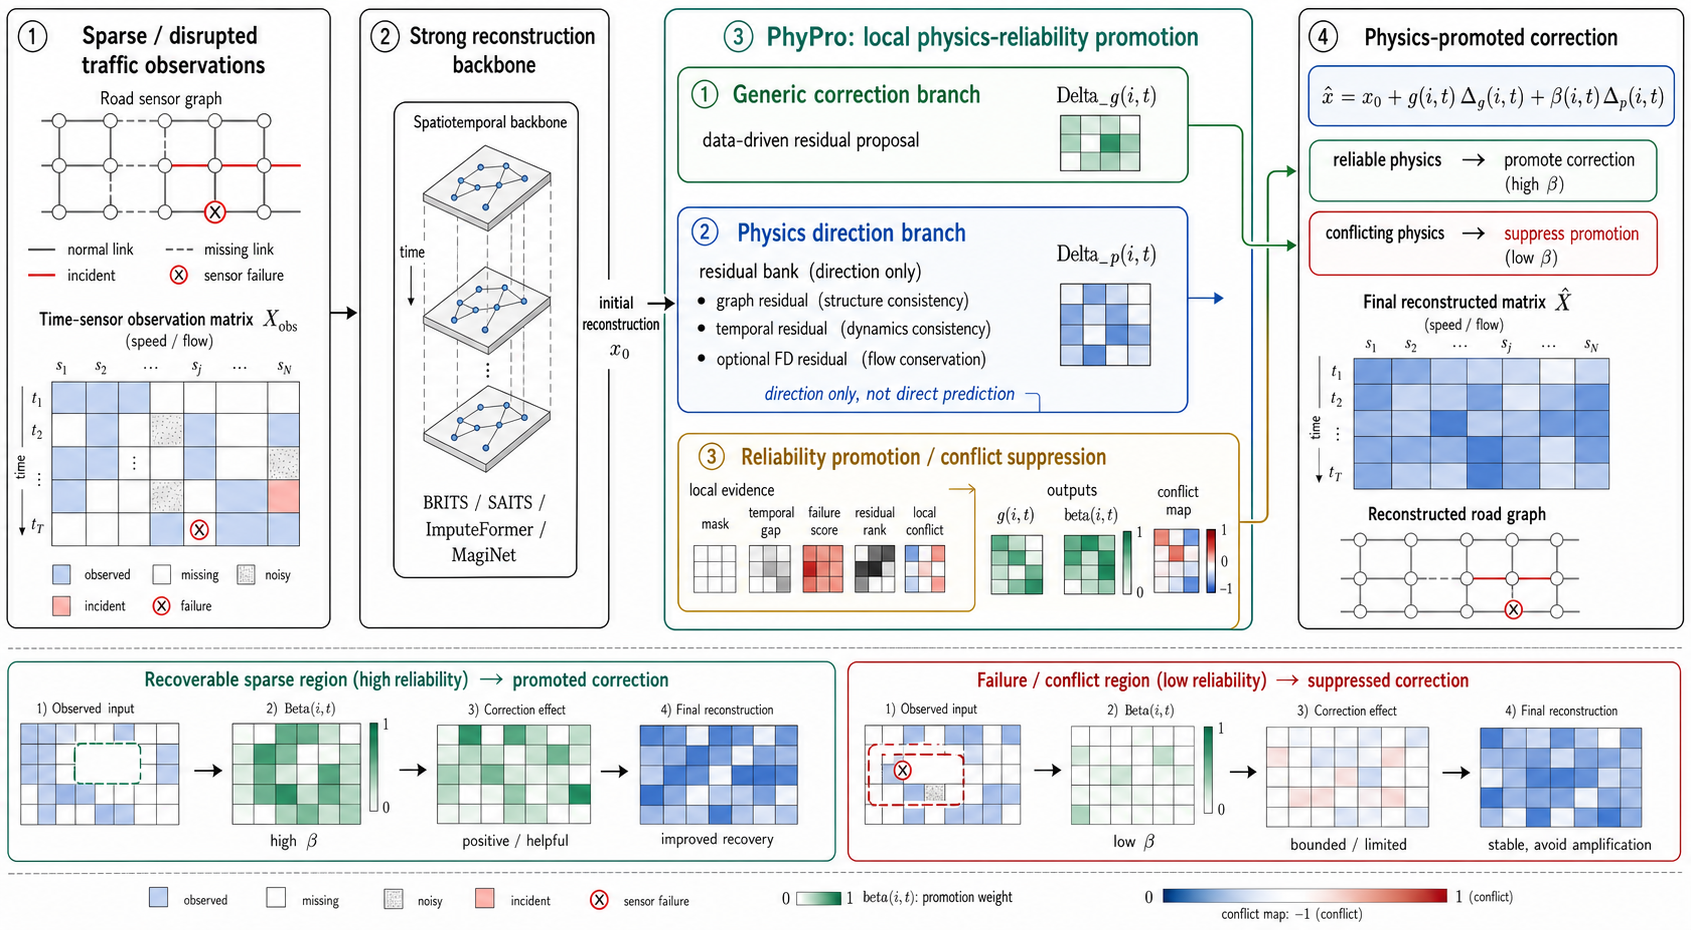
\includegraphics[width=\textwidth]{figures/figure_phypro_mechanism.png}
  \caption{Overview of PhyPro. A strong backbone first produces an initial reconstruction. PhyPro then learns a generic residual correction and a physics-aligned direction, while local evidence determines whether physics should promote or suppress the correction.}
  \label{fig:mechanism}
\end{figure}

\subsection{Local Evidence Bank}
For each $(t,i)$, PhyPro constructs an evidence vector
\begin{equation}
  \mathbf{e}_{t,i}
  =
  \left[
  m_{t,i},
  q_{t,i},
  f_{t,i},
  r^{graph}_{t,i},
  r^{temp}_{t,i},
  u_{t,i},
  c_{t,i}
  \right],
\end{equation}
where $m_{t,i}$ denotes local observation availability, $q_{t,i}$ measures temporal gap or local sparsity, $f_{t,i}$ is a failure-mode score, $r^{graph}_{t,i}$ and $r^{temp}_{t,i}$ are graph and temporal residual features, $u_{t,i}$ is an observed-error proxy when available from validation-like evidence, and $c_{t,i}$ is a local conflict cue. The failure score is high when a sensor has persistent missingness, while the conflict cue is high when physical residuals, local discontinuity, or graph-neighborhood disagreement suggest that physics may be misleading.

The graph residual direction is computed from the backbone estimate:
\begin{equation}
  d^{graph}_{t,i}
  =
  x_{0,t,i}
  -
  \sum_{j}\bar{A}_{ij}x_{0,t,j},
\end{equation}
where $\bar{A}$ is a normalized adjacency matrix. The temporal direction is
\begin{equation}
  d^{temp}_{t,i}
  =
  x_{0,t,i}-x_{0,t-1,i}.
\end{equation}
For multivariate traffic states, an optional flow-density-speed residual can be included:
\begin{equation}
  r^{fd}_{t,i}
  =
  \frac{\hat{q}_{t,i}-\hat{\rho}_{t,i}\hat{v}_{t,i}}{s_{fd}},
\end{equation}
where the variables are computed in inverse-normalized physical scale and $s_{fd}$ is a robust scale factor. If a dataset is speed-only, unavailable residual components are masked out rather than forced into the model.

\subsection{Physics-Reliability Promoted Correction}
The generic correction branch uses data-driven features to produce a bounded residual:
\begin{equation}
  \Delta^{g}_{t,i}
  =
  b\cdot \tanh\left(f_g(\mathbf{z}^{g}_{t,i})\right),
\end{equation}
where $b$ is a correction bound and $\mathbf{z}^{g}_{t,i}$ contains backbone value, mask, temporal, graph, and local error-proxy features. The physics-aligned direction is constructed as
\begin{equation}
  \Delta^{p}_{t,i}
  =
  b\cdot \tanh\left(
  \lambda_g d^{graph}_{t,i}
  +
  \lambda_t d^{temp}_{t,i}
  \right),
\end{equation}
with $\lambda_g+\lambda_t=1$. In the implementation, $\lambda_g=0.6$ and $\lambda_t=0.4$.

The promotion branch receives reliability features and outputs
\begin{equation}
  g_{t,i}=g_{\min}+(1-g_{\min})\sigma(f_{gate}(\mathbf{e}_{t,i})),
  \quad
  \beta^{raw}_{t,i}=\sigma(f_{\beta}(\mathbf{e}_{t,i})).
\end{equation}
To prevent physics from amplifying abnormal local states, PhyPro applies conflict suppression:
\begin{equation}
  \beta_{t,i}
  =
  \beta^{raw}_{t,i}
  \left(1-\lambda_c C_{t,i}\right),
  \quad
  C_{t,i}\in[0,1],
\end{equation}
where $C_{t,i}$ combines failure score, residual rank, observed-error proxy, and spatial-gap rank. This mechanism is the central difference between PhyPro and a generic adapter. A generic adapter learns how to correct; PhyPro additionally learns when physics should promote that correction and when it should be suppressed. Algorithm~\ref{alg:phypro} gives the local inference rule in the same notation.

\begin{algorithm}[t]
\caption{Local physics-reliability promoted correction}
\label{alg:phypro}
\begin{algorithmic}[1]
\Require Backbone estimate $X_0$, observation mask $M$, graph $A$, target region $\Omega$, correction bound $b$
\Ensure Reconstruction $\hat{X}$, gate map $G$, promotion map $B$
\For{$(t,i)\in\Omega$}
  \State $\mathbf{z}^{g}_{t,i}\gets [x_{0,t,i}, M_{t,i}, q_{t,i}, d^{graph}_{t,i}, d^{temp}_{t,i}, u_{t,i}]$
  \State $\mathbf{e}_{t,i}\gets [M_{t,i}, q_{t,i}, f_{t,i}, \rho_{t,i}, u_{t,i}, C_{t,i}]$
  \State $\Delta^{g}_{t,i}\gets b\,\tanh(f_g(\mathbf{z}^{g}_{t,i}))$
  \State $\Delta^{p}_{t,i}\gets b\,\tanh(0.6\,d^{graph}_{t,i}+0.4\,d^{temp}_{t,i})$
  \State $g_{t,i}\gets g_{\min}+(1-g_{\min})\sigma(f_{gate}(\mathbf{e}_{t,i}))$
  \State $\beta^{raw}_{t,i}\gets\sigma(f_{\beta}(\mathbf{e}_{t,i}))$
  \State $\beta_{t,i}\gets\beta^{raw}_{t,i}(1-\lambda_c C_{t,i})$
  \State $\hat{x}_{t,i}\gets x_{0,t,i}+g_{t,i}\Delta^g_{t,i}+\beta_{t,i}\Delta^p_{t,i}$
\EndFor
\State \Return $\hat{X},G,B$
\end{algorithmic}
\end{algorithm}

\subsection{Training Objective}
PhyPro is trained on target reconstruction regions using
\begin{equation}
  \mathcal{L}
  =
  \mathcal{L}_{rec}
  +\lambda_g\mathcal{L}_{gate}
  +\lambda_p\mathcal{L}_{promo}
  +\lambda_h\mathcal{L}_{harm}
  +\lambda_s\mathcal{L}_{shrink}.
\end{equation}
The reconstruction term is the mean absolute error on missing or disrupted entries. The gate and promotion losses use contrastive utility labels derived from local error comparisons during training. The generic correction is useful when it improves over the backbone, and physics promotion is useful when a physics-aligned probe improves over the generic correction. The harm term penalizes corrections that exceed the better of the backbone and generic correction:
\begin{equation}
  \mathcal{L}_{harm}
  =
  \mathbb{E}_{(t,i)\in\Omega}
  \left[
  w_{t,i}
  \max
  \left(
  0,
  |\hat{x}_{t,i}-x_{t,i}|-
  \min(|x_{0,t,i}-x_{t,i}|,|x_{0,t,i}+\Delta^g_{t,i}-x_{t,i}|)
  \right)
  \right],
\end{equation}
where $w_{t,i}$ increases with failure and residual-conflict evidence. This term makes the correction conservative in regions where an incorrect update may persist or amplify a local abnormal state.

\section{Experiments}

\subsection{Datasets and Disruption Protocols}
We evaluate PhyPro on five public traffic datasets: PEMS03, PEMS04, PEMS08, PEMS-BAY, and METR-LA. PEMS03, PEMS04, and PEMS08 provide freeway traffic measurements from different sensor networks, while PEMS-BAY and METR-LA are widely used speed-based traffic sensor datasets. The use of both multivariate and speed-only datasets tests whether the reliability-promotion idea generalizes beyond a single residual definition.

We consider three reconstruction protocols. Random missing removes observed entries uniformly and tests sparse point-wise reconstruction. Sensor failure removes selected sensors over the evaluated window and represents persistent detector malfunction. Incident perturbation injects local disrupted traffic states and tests whether the model avoids unreliable local corrections under abnormal dynamics. All main results use three random seeds.

\subsection{Baselines and Backbones}
PhyPro is attached to four strong and diverse reconstruction backbones: BRITS \citep{cao2018brits}, SAITS \citep{du2023saits}, ImputeFormer \citep{liu2024imputeformer}, and MagiNet \citep{liu2025maginet}. BRITS represents bidirectional recurrent imputation, SAITS represents self-attention-based temporal imputation, ImputeFormer represents transformer-style masked spatiotemporal imputation, and MagiNet represents mask-aware graph repair. This selection avoids testing only minor variants of one architecture family.

We report two types of comparisons. The first compares each backbone with the same backbone enhanced by PhyPro. The second compares PhyPro with plug-in baselines under the same backbone outputs: Generic Adapter, Calibration Guard, and Failure/Anomaly Guard. Generic Adapter follows the residual-adapter idea used in parameter-efficient adaptation \citep{houlsby2019adapter}; Calibration Guard follows confidence calibration \citep{guo2017calibration}; and Failure/Anomaly Guard follows failure detection and selective prediction principles \citep{hendrycks2017baseline,geifman2019selectivenet}. This protocol isolates whether PhyPro improves because of physics-reliability promotion rather than because an additional adapter was added.

The primary metric is masked MAE on the target missing or disrupted region:
\begin{equation}
  \mathrm{MAE}_{\Omega}
  =
  \frac{1}{|\Omega|}
  \sum_{(t,i,c)\in\Omega}
  |\hat{x}_{t,i,c}-x_{t,i,c}|.
\end{equation}
RMSE and MAPE are recorded but not used for the main ranking. Unless otherwise stated, experiments use correction bound $b=0.20$, gate floor $g_{\min}=0.95$, and conflict coefficient $\lambda_c=0.75$.

\subsection{Main Results}
Table~\ref{tab:main_mae} reports the main paired comparison. PhyPro improves all four backbones on average. Across 180 paired runs, the mean masked MAE decreases from 0.3804 to 0.3441, corresponding to a 10.58\% average reduction. The gain is larger under random missing and incident perturbation than under sensor failure, which agrees with the motivation that physical and graph-temporal evidence is more identifiable in recoverable sparse regions than in persistent node-level absence.

\begin{table}[!htbp]
\centering
\scriptsize
\setlength{\tabcolsep}{1.8pt}
\caption{Main masked MAE ($\downarrow$) results. Each backbone is compared with the same backbone enhanced by PhyPro. Ours denotes the PhyPro-enhanced variant.}
\label{tab:main_mae}
\resizebox{0.96\linewidth}{!}{%
\begin{tabular}{@{}llcccccccc@{}}
\toprule
Dataset & Scenario & \multicolumn{2}{c}{BRITS} & \multicolumn{2}{c}{ImputeFormer} & \multicolumn{2}{c}{MagiNet} & \multicolumn{2}{c}{SAITS} \\
\cmidrule(lr){3-4}\cmidrule(lr){5-6}\cmidrule(lr){7-8}\cmidrule(lr){9-10}
 & & Base $\downarrow$ & Ours $\downarrow$ & Base $\downarrow$ & Ours $\downarrow$ & Base $\downarrow$ & Ours $\downarrow$ & Base $\downarrow$ & Ours $\downarrow$ \\
\midrule
METR-LA & Incident & 0.4605 & \textbf{0.4235} & 0.3671 & \textbf{0.3455} & 0.3766 & \textbf{0.3577} & 0.4725 & \textbf{0.4445} \\
METR-LA & Random & 0.4462 & \textbf{0.4080} & 0.3371 & \textbf{0.3181} & 0.3576 & \textbf{0.3363} & 0.4575 & \textbf{0.4290} \\
METR-LA & Failure & 0.5643 & \textbf{0.5388} & 0.7678 & \textbf{0.7067} & 0.7436 & \textbf{0.7238} & 0.5014 & \textbf{0.4908} \\
PEMS-BAY & Incident & 0.4143 & \textbf{0.3644} & 0.2878 & \textbf{0.2589} & 0.2632 & \textbf{0.2373} & 0.4245 & \textbf{0.3740} \\
PEMS-BAY & Random & 0.4041 & \textbf{0.3511} & 0.2785 & \textbf{0.2471} & 0.2454 & \textbf{0.2164} & 0.4170 & \textbf{0.3617} \\
PEMS-BAY & Failure & 0.5661 & \textbf{0.5508} & 0.7451 & \textbf{0.7149} & 0.7281 & \textbf{0.7006} & 0.5315 & \textbf{0.5150} \\
PEMS03 & Incident & 0.2887 & \textbf{0.2535} & 0.1832 & \textbf{0.1666} & 0.1734 & \textbf{0.1593} & 0.2842 & \textbf{0.2506} \\
PEMS03 & Random & 0.2674 & \textbf{0.2309} & 0.1570 & \textbf{0.1390} & 0.1501 & \textbf{0.1346} & 0.2639 & \textbf{0.2270} \\
PEMS03 & Failure & 0.5335 & \textbf{0.5134} & 0.8446 & \textbf{0.7899} & 0.6747 & \textbf{0.6691} & 0.4975 & \textbf{0.4838} \\
PEMS04 & Incident & 0.2145 & \textbf{0.1903} & 0.1906 & \textbf{0.1755} & 0.1723 & \textbf{0.1634} & 0.2150 & \textbf{0.1951} \\
PEMS04 & Random & 0.1886 & \textbf{0.1645} & 0.1663 & \textbf{0.1496} & 0.1566 & \textbf{0.1458} & 0.1852 & \textbf{0.1657} \\
PEMS04 & Failure & 0.4528 & \textbf{0.4075} & 0.7120 & \textbf{0.6347} & 0.5912 & \textbf{0.5711} & 0.4150 & \textbf{0.3873} \\
PEMS08 & Incident & 0.2890 & \textbf{0.2699} & 0.1638 & \textbf{0.1608} & 0.1494 & \textbf{0.1468} & 0.2985 & \textbf{0.2840} \\
PEMS08 & Random & 0.2784 & \textbf{0.2628} & 0.1452 & \textbf{0.1417} & 0.1333 & \textbf{0.1300} & 0.2841 & \textbf{0.2739} \\
PEMS08 & Failure & 0.4257 & \textbf{0.4148} & 0.6324 & \textbf{0.6115} & 0.5002 & \textbf{0.4989} & 0.4356 & \textbf{0.4225} \\
\bottomrule
\end{tabular}
}
\end{table}

\subsection{Plug-in Comparison and Significance}
Table~\ref{tab:plugin} compares PhyPro with other plug-in adapters. Generic Adapter already improves the backbone by learning a data-driven residual correction. PhyPro further improves over it by adding physics-reliability promotion and conflict suppression. Paired tests in Table~\ref{tab:significance} show that the improvements are statistically stable across matched dataset, scenario, seed, and backbone settings.

\begin{table}[!htbp]
\centering
\caption{Plug-in comparison by disruption scenario. Values are masked MAE ($\downarrow$).}
\label{tab:plugin}
\resizebox{0.96\linewidth}{!}{%
\begin{tabular}{lccccc}
\toprule
Setting & Backbone $\downarrow$ & Generic Adapter $\downarrow$ & Calibration Guard $\downarrow$ & Failure/Anomaly Guard $\downarrow$ & PhyPro (Ours) $\downarrow$ \\
\midrule
Overall & 0.3804 $\pm$ 0.1881 & 0.3496 $\pm$ 0.1830 & 0.3556 $\pm$ 0.1843 & 0.3550 $\pm$ 0.1841 & \textbf{0.3441 $\pm$ 0.1805} \\
Random missing & 0.2643 & 0.2309 & 0.2375 & 0.2372 & \textbf{0.2261} \\
Sensor failure & 0.5930 & 0.5661 & 0.5712 & 0.5698 & \textbf{0.5583} \\
Incident perturbation & 0.2839 & 0.2517 & 0.2582 & 0.2582 & \textbf{0.2479} \\
\bottomrule
\end{tabular}
}
\end{table}

\begin{table}[!htbp]
\centering
\caption{Paired significance tests for PhyPro. Comparisons use matched dataset, scenario, seed, and backbone settings.}
\label{tab:significance}
\resizebox{0.96\linewidth}{!}{%
\begin{tabular}{lccc}
\toprule
Comparison & Mean improvement $\uparrow$ & Paired $t$-test $p$ $\downarrow$ & Wilcoxon $p$ $\downarrow$ \\
\midrule
PhyPro vs Backbone & \textbf{10.58\%} & \textbf{$2.29{\times}10^{-54}$} & \textbf{$2.73{\times}10^{-31}$} \\
PhyPro vs Generic Adapter & 1.58\% & $1.01{\times}10^{-21}$ & $7.02{\times}10^{-28}$ \\
PhyPro vs Calibration Guard & 3.46\% & $3.12{\times}10^{-38}$ & $1.09{\times}10^{-30}$ \\
PhyPro vs Failure/Anomaly Guard & 3.29\% & $8.13{\times}10^{-36}$ & $1.33{\times}10^{-30}$ \\
\bottomrule
\end{tabular}
}
\end{table}

\subsection{Ablation Study}
Table~\ref{tab:ablation} reports a selected ablation on PEMS08 using SAITS and MagiNet over three scenarios and three seeds. The residual/evidence bank is the most important component: removing it brings the model close to the backbone. Generic correction alone is helpful, but full PhyPro achieves lower MAE by adding physics-reliability promotion. Conflict and failure terms have smaller average effects because their benefit is scenario-dependent, especially under sensor failure and incident-like regions.

\begin{table}[!htbp]
\centering
\small
\caption{Selected ablation results on PEMS08. Values are masked MAE ($\downarrow$); internal diagnostic variants are omitted from the main text.}
\label{tab:ablation}
\resizebox{0.86\linewidth}{!}{%
\begin{tabular}{lccc}
\toprule
Variant & Masked MAE $\downarrow$ & Gate mean $\uparrow$ & Promotion mean $\uparrow$ \\
\midrule
Backbone & 0.2988 & -- & -- \\
Generic correction only & 0.2863 & 1.0000 & -- \\
Full PhyPro (Ours) & \textbf{0.2786} & 0.9566 & 0.4872 \\
w/o physics promotion & 0.2789 & 0.9567 & 0.0779 \\
w/o residual/evidence bank & 0.2975 & 0.9682 & 0.3322 \\
w/o conflict suppression & 0.2788 & 0.9572 & 0.5500 \\
w/o failure evidence & 0.2786 & 0.9568 & 0.5230 \\
\bottomrule
\end{tabular}
}
\end{table}

\subsection{Parameter Sensitivity}
Table~\ref{tab:param_sensitivity} reports a small sensitivity check for the gate floor and conflict coefficient. The table is used only to justify the final default configuration. The best setting among the tested pairs is $g_{\min}=0.95$ and $\lambda_c=0.75$.

\begin{table}[!htbp]
\centering
\caption{Parameter sensitivity for the final PhyPro configuration.}
\label{tab:param_sensitivity}
\resizebox{0.86\linewidth}{!}{%
\begin{tabular}{ccccc}
\toprule
Gate floor & Conflict coefficient & Masked MAE $\downarrow$ & Gate mean $\uparrow$ & Promotion mean $\uparrow$ \\
\midrule
0.95 & 0.75 & \textbf{0.3143} & 0.9730 & 0.4252 \\
0.90 & 0.50 & 0.3170 & 0.9461 & 0.4597 \\
0.95 & 0.50 & 0.3177 & 0.9730 & 0.4599 \\
0.90 & 0.75 & 0.3219 & 0.9461 & 0.4251 \\
\bottomrule
\end{tabular}
}
\end{table}

\subsection{Interpretability Analysis}
Figures~\ref{fig:case_obs}--\ref{fig:case_corr} visualize a representative PEMS-BAY case under random missing. The panels show the observation pattern, initial backbone reconstruction, PhyPro reconstruction, error reduction, learned correction, physics direction, promotion weight, and failure evidence. The example illustrates how PhyPro exposes the mechanism behind the update: the final correction is not a black-box residual, but a combination of a learned correction and a physics-aligned promotion term.

\begin{figure}[!htbp]
  \centering
  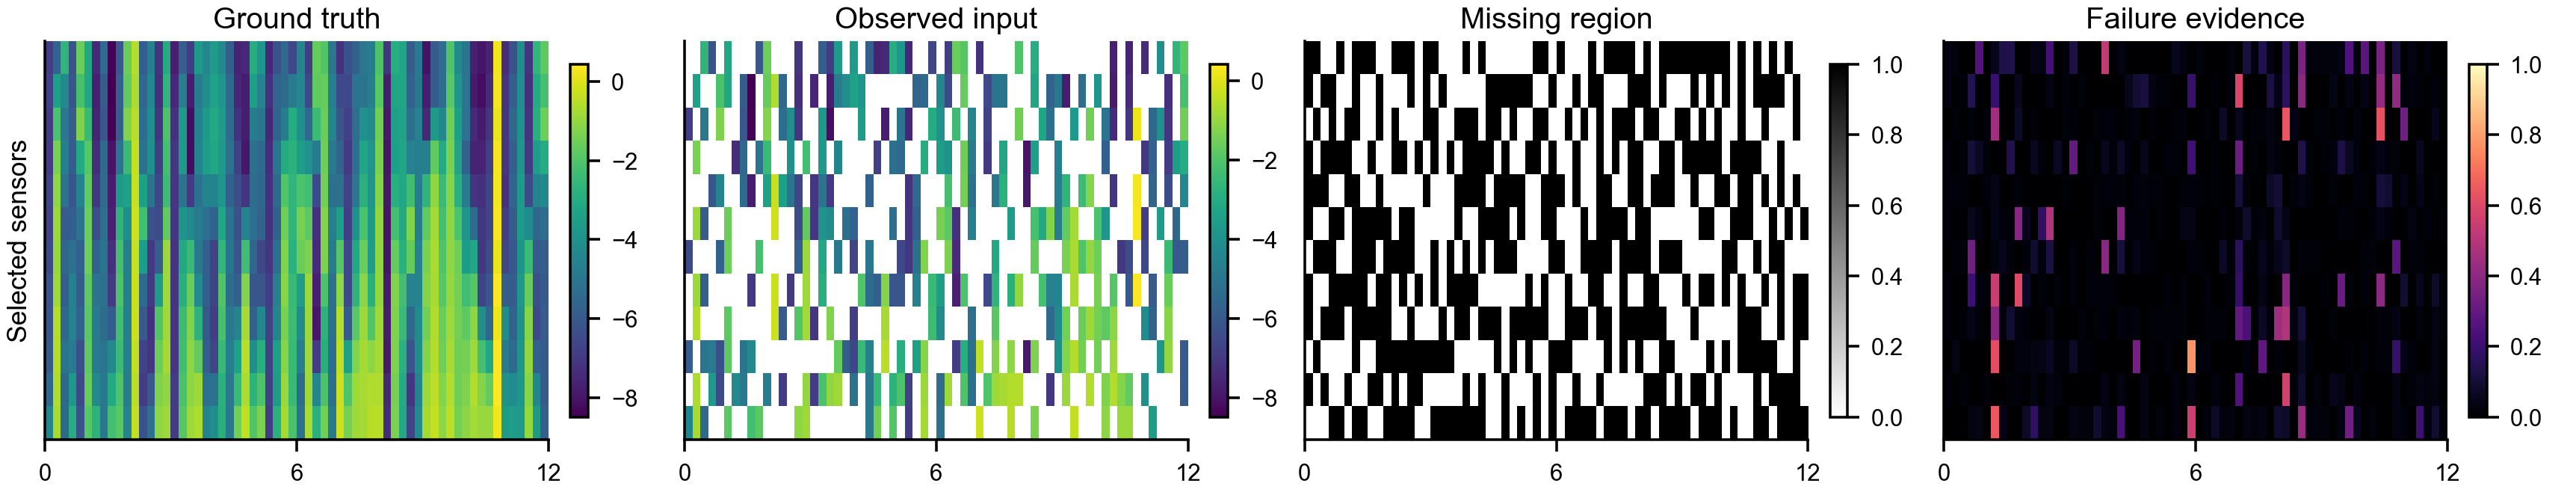
\includegraphics[width=\textwidth]{figures/figure_phypro_case_a.png}
  \caption{Representative PhyPro reconstruction case on PEMS-BAY under random missing with 50\% missingness: observation and disruption evidence.}
  \label{fig:case_obs}
\end{figure}

\begin{figure}[!htbp]
  \centering
  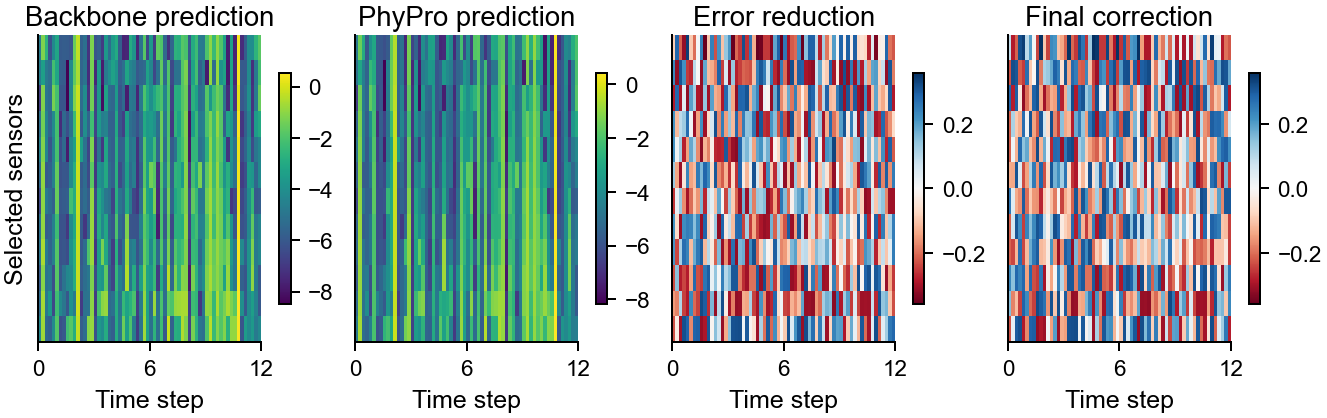
\includegraphics[width=\textwidth]{figures/figure_phypro_case_b.png}
  \caption{Representative PhyPro reconstruction case: initial reconstruction, PhyPro reconstruction, and error reduction. PhyPro reduces masked MAE from 0.2457 to 0.2070 in this case.}
  \label{fig:case_recon}
\end{figure}

\begin{figure}[!htbp]
  \centering
  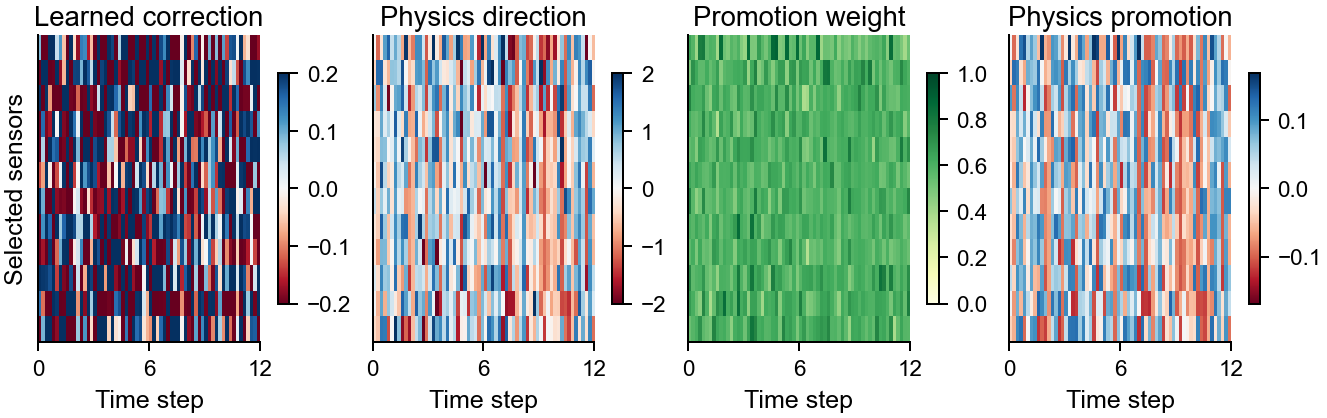
\includegraphics[width=\textwidth]{figures/figure_phypro_case_c.png}
  \caption{Representative PhyPro reconstruction case: learned correction, physics direction, promotion weight, and failure evidence.}
  \label{fig:case_corr}
\end{figure}

\begin{table}[!htbp]
\centering
\caption{Region-level mechanism statistics. The table reports mechanism variables only and does not repeat main-table gains.}
\label{tab:interpretability}
\resizebox{0.96\linewidth}{!}{%
\begin{tabular}{lccccc}
\toprule
Region & Masked MAE $\downarrow$ & Reliability gate $\uparrow$ & Promotion mean $\uparrow$ & $|\Delta_g|$ mean $\downarrow$ & Failure score $\uparrow$ \\
\midrule
Random missing & \textbf{0.2261} & 0.9503 & 0.5264 & \textbf{0.0757} & 0.0764 \\
Sensor failure & 0.5583 & 0.9545 & 0.5512 & 0.1185 & 0.7825 \\
Incident/disrupted & 0.2479 & 0.9503 & 0.5233 & 0.0759 & 0.0764 \\
\bottomrule
\end{tabular}
}
\end{table}

\subsection{Robustness to Missing Rates}
Table~\ref{tab:missing_rate} reports a quick missing-rate robustness check on PEMS08, PEMS-BAY, and METR-LA using SAITS and MagiNet. PhyPro remains the best plug-in across 30\%, 50\%, and 70\% random missing rates. The margin decreases at 70\% missingness, which is expected because both data-driven evidence and physics-aligned directions become less identifiable under extreme sparsity.

\begin{table}[!htbp]
\centering
\small
\caption{Missing-rate robustness under random missing protocols.}
\label{tab:missing_rate}
\resizebox{0.96\linewidth}{!}{%
\begin{tabular}{lccccc}
\toprule
Missing rate & Backbone $\downarrow$ & Generic Adapter $\downarrow$ & Calibration Guard $\downarrow$ & Failure/Anomaly Guard $\downarrow$ & PhyPro $\downarrow$ \\
\midrule
30\% & 0.3173 $\pm$ 0.1124 & 0.2960 $\pm$ 0.1020 & 0.3019 $\pm$ 0.1050 & 0.3051 $\pm$ 0.1072 & \textbf{0.2815 $\pm$ 0.0974} \\
50\% & 0.3317 $\pm$ 0.1140 & 0.3097 $\pm$ 0.1035 & 0.3147 $\pm$ 0.1065 & 0.3160 $\pm$ 0.1078 & \textbf{0.2988 $\pm$ 0.1002} \\
70\% & 0.3583 $\pm$ 0.1164 & 0.3372 $\pm$ 0.1085 & 0.3422 $\pm$ 0.1109 & 0.3427 $\pm$ 0.1113 & \textbf{0.3307 $\pm$ 0.1080} \\
\bottomrule
\end{tabular}
}
\end{table}

\subsection{Complexity Analysis}
PhyPro is lightweight because it operates on local evidence after the backbone output is produced. The module adds 23,365 trainable parameters for all datasets. Table~\ref{tab:complexity} reports the extra forward time, which remains below 2.6 ms per batch on the tested graphs.

\begin{table}[!htbp]
\centering
\small
\caption{Runtime overhead of PhyPro. Runtime is extra forward time per batch with shape $16{\times}12{\times}N{\times}1$.}
\label{tab:complexity}
\begin{tabular}{lcc}
\toprule
Dataset & Nodes & Extra time (ms) $\downarrow$ \\
\midrule
PEMS03 & 358 & 2.52 \\
PEMS04 & 307 & 1.93 \\
PEMS08 & 170 & \textbf{0.99} \\
PEMS-BAY & 325 & 2.11 \\
METR-LA & 207 & 1.21 \\
\bottomrule
\end{tabular}
\end{table}

\section{Discussion}
PhyPro differs from fixed physics-informed losses in both objective and failure mode. A fixed physics loss assumes that the same residual should guide every sensor and time step. PhyPro assumes the opposite: physical evidence is useful only when local observations, graph context, temporal behavior, and residual consistency indicate that it is reliable. This explains why the method uses physics as a promotion direction and conflict-aware reliability signal rather than as a universally enforced constraint. The paired improvements over Generic Adapter show that the benefit is not merely the presence of an additional residual correction head; physics-reliability evidence provides a small but stable advantage on top of a strong generic correction.

The sensor-failure scenario yields smaller gains than random missing and incident perturbation. This result is consistent with the problem structure. In sensor failure, an entire node can be unobserved for a long interval, so both local temporal evidence and physical residuals become less identifiable. Neighboring sensors may not fully determine the failed node, and aggressive correction can propagate a wrong estimate. PhyPro therefore behaves more conservatively in this setting, as reflected by high failure scores and bounded correction magnitudes. The result should not be interpreted as physics being useless under sensor failure; rather, it shows that persistent node-level absence is the hardest case for local reliability promotion.

PhyPro is designed as a plug-in rather than a new backbone because the studied gap is not simply backbone capacity. Strong backbones already model temporal recurrence, self-attention, transformer masking, or graph repair. The missing component is a local mechanism that decides how a correction should interact with physical evidence. A plug-in design makes this mechanism compatible with different reconstruction cores, keeps the added cost small, and allows the same reliability and promotion maps to be inspected across backbones. This positioning also limits the claim: PhyPro does not replace the need for strong reconstruction models, but it improves their local reliability under sparse and disrupted sensing.

\section{Conclusion}
This paper introduced PhyPro, a physics-reliability promoted correction framework for robust traffic state reconstruction. PhyPro addresses the local physical-misguidance problem by replacing globally enforced physics with local reliability-controlled promotion. Given a backbone reconstruction, it combines a data-driven correction proposal, a physics-aligned direction, and conflict-aware promotion weights to decide when physics should strengthen or suppress local corrections.

Experiments on five public datasets, three disruption protocols, three random seeds, and four diverse reconstruction backbones show that PhyPro consistently improves masked MAE while adding only 23,365 trainable parameters. The plug-in comparison, ablation, missing-rate robustness, significance tests, complexity analysis, and visual explanations jointly support the central claim: physics is most useful for robust traffic reconstruction when it serves as local reliability evidence for correction, not as a fixed global constraint.

\section*{Data Availability}
The experiments use public traffic benchmark datasets. PEMS03, PEMS04, and PEMS08 are loaded from public PEMS benchmark mirrors, PEMS-BAY is loaded from the Hugging Face dataset \texttt{MintBruce/SkyTraffic}, and METR-LA is loaded from the Hugging Face dataset \texttt{witgaw/METR-LA}. The repository documents the exact loaders and preprocessing scripts used in the experiments. Raw datasets are not redistributed by this manuscript.

\section*{Code Availability}
The anonymized implementation and reproduction scripts are available at: \url{https://anonymous.4open.science/r/PhyPRO}.

\bibliographystyle{elsarticle-num}
\bibliography{references}

\end{document}
